\documentclass{article}

\usepackage{tikz}

\usetikzlibrary{arrows,automata,positioning}

\begin{document}

Partial DFA recognizing the language:

``\texttt{ *(int|if|[a-z]+) }'' \\

Alphabet = ``[ a-z]''

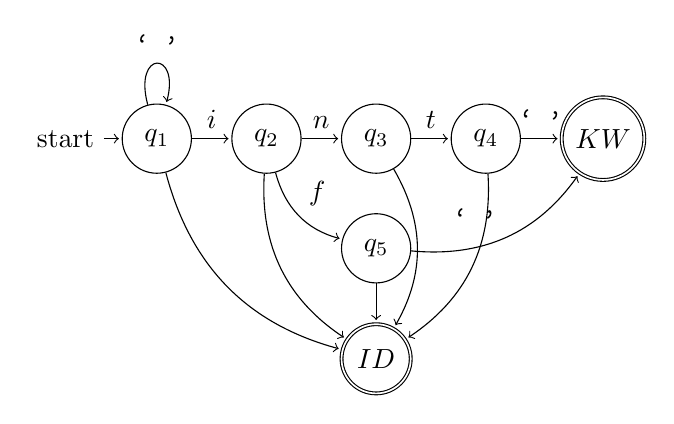
\begin{tikzpicture}[scale=0.5,shorten >=1pt,node distance=0.5cm,auto]
    \node[state,initial left] (q1) {$q_1$};
    \node[state] (q2) [right=of q1] {$q_2$};
    \node[state] (q3) [right=of q2] {$q_3$};
    \node[state] (q4) [right=of q3] {$q_4$};
    \node[state,accepting] (kw) [right=of q4] {$KW$};
    \node[state] (q5) [below=of q3] {$q_5$};
    \node[state,accepting] (id) [below=of q5] {$ID$};
    \path[->]
    (q1) edge [loop above] node {\texttt{` '}} (q1)
         edge node {$i$} (q2)
         edge [bend right] node {} (id)
    (q2) edge node {$n$} (q3)
         edge [bend right] node {$f$} (q5)
         edge [bend right] node {} (id)
    (q3) edge node {$t$} (q4)
         edge [bend left] node {} (id)
    (q4) edge node {\texttt{` '}} (kw)
         edge [bend left] node {} (id)
    (q5) edge [bend right] node {\texttt{` '}} (kw)
         edge node {} (id);
\end{tikzpicture}

\end{document}
